Face Generation is an important field in the market. It is used widely in missing people organizations or police stations, however it is not automated, using artists to draw the faces from their descriptions. Retratista is the first automated product in that field, so it can be used faster and more accurate. Retratista, also, offers face refinement, which is offered by many mobile applications just to enhance or edit taken photos for entertainment, not critical issues like the ones we target. 

\subsection{Targeted Customers}
Our Project is directed to all governmental and volunteering organizations, that need to generate identical faces of missing people from bare human description of their facial features.
Also, it can be used to identify the ancient kings and queens faces from historical descriptions.
We can categorize the different target companies into the following :
\begin{itemize}
    \item \textbf{Criminal identification from witnesses descriptions :}
        \begin{itemize}
            \item INTERPOL.
            \item Different Police Stations.
        \end{itemize}
    \item \textbf{Missing People organizations like :}
        \begin{itemize}
            \item International Center for Missing and Exploited Children. (ref: \link{https://www.icmec.org})
            \item International Red Cross and Red Crescent Movement. (ref: \link{https://www.icrc.org})
            \item International Commission on Missing Persons \emph{ICMP} (ref: \link{https://www.icmp.int})
            \item Missing Persons Support Center. (ref: \link{https://www.mpsupportcenter.org})
            \item Others.
        \end{itemize}
    \item \textbf{Historical Characters Identification :}
        \begin{itemize}
            \item Archaeological and Historical Research Facilities.
        \end{itemize}
\end{itemize}

\subsection{Market Survey}

Retratista is the first innovative product that offers face portrait generation in an automated way. Consequently, we have no direct market competitors. Competitor products depend only on image refinement using limited number of features to manipulate a given face. We have both image generation and refinement using $32$ facial features for generation and $38$ facial features for refinement, which exceed the number of facial features targeted by any competitor. Besides that, our purpose is more important than just entertainment. Our biggest competitor is \emph{FaceApp}, followed by \emph{PicsArt}, \emph{Facetune2} and \emph{Booth Apps}.

\subsubsection{FaceApp}
\emph{FaceApp} (ref: \link{https://www.faceapp.com/}) is considered image and video editing mobile application, it generates highly realistic transformations of human faces in photographs using \emph{AI} and \emph{Neural Networks}. The limitation of the application compared to us is that it's only used for refinement using $14$ facial feature, which might not be enough for generating face from scratch. Figure \ref{fig:faceApp} shows an example of changing a face age using \emph{FaceApp}. The considered facial features include \emph{different styles of beard}, \emph{hair color and style}, \emph{makeup filters}, \emph{blemishes removal}, \emph{eyes color}, \emph{gender}, \emph{age}, \emph{glasses}, \emph{smile} and \emph{lips, eyes and nose size}.

\begin{figure}[H]
    \centering
    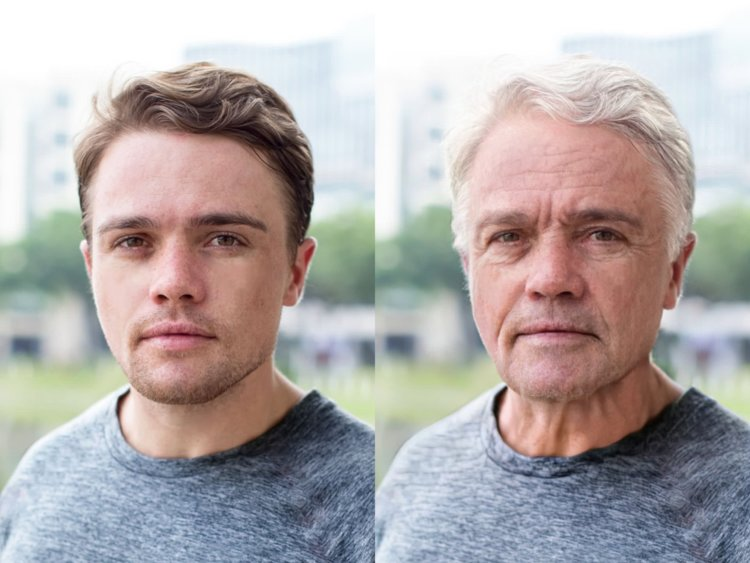
\includegraphics[width=0.5\textwidth]{images/FaceApp.jpg}
    \caption{Changing age using FaceApp application.}
    \label{fig:faceApp}
\end{figure}

\subsubsection{PicsArt}
\emph{PicsArt} (ref: \link{https://picsart.com/}) is a company that develops online photo and video editing applications, with a social creative community. The platform allows users to take and edit pictures and videos and draw with layers. It only allows $9$ facial features refinement, so it's also not the best choice for image generation. Figure \ref{fig:picsArt} shows an example of hair color change using \emph{PicsArt} platform. The considered facial features include \emph{face size}, \emph{lips, eyes and nose size}, \emph{eye-bags}, \emph{hair color}, \emph{eyes color}, \emph{blemishes removal} and \emph{teeth whitening}.

\begin{figure}[H]
    \centering
    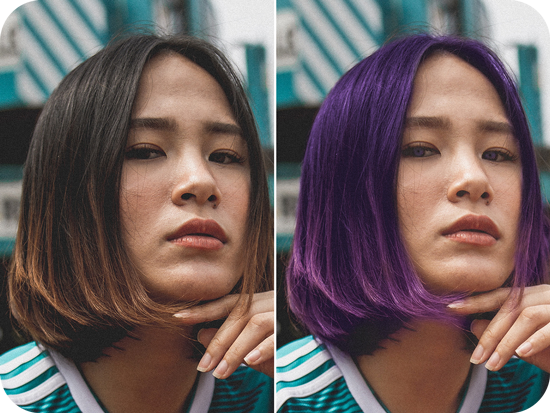
\includegraphics[width=0.5\textwidth]{images/picsArt.png}
    \caption{Image refinement using PicsArt application.}
    \label{fig:picsArt}
\end{figure}

\subsubsection{Facetune2}
\emph{Facetune2} (ref: \link{https://www.facetuneapp.com/}) is a photo editing application. It's commonly used to enhance the portrait o selfie images and offers $7$ feature refinements. Figure \ref{fig:FaceTune2} shows an example of image refinement using \emph{Facetune2} application. The considered facial features include \emph{face shape}, \emph{skin smoothing}, \emph{makeup}, \emph{teeth whitening} and \emph{eyes and nose size}.

\begin{figure}[H]
    \centering
    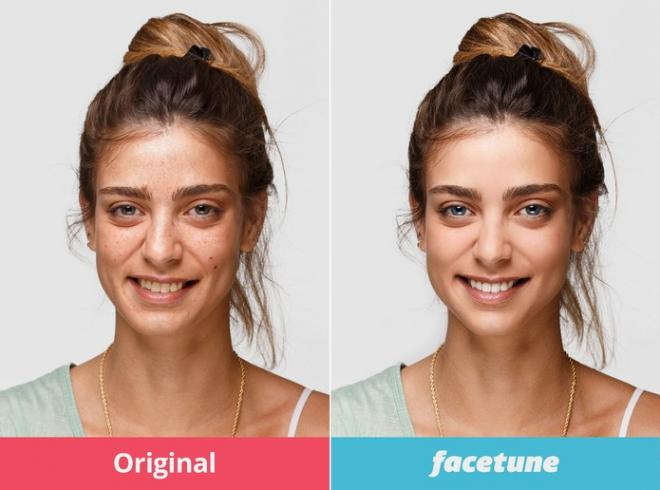
\includegraphics[width=0.5\textwidth]{images/FaceTune.jpg}
    \caption{Image refinement using Facetune2 application.}
    \label{fig:FaceTune2}
\end{figure}

\subsubsection{Booth Apps}
\emph{Booth Apps} are a collection of applications for image or video editing and enhancement, can add animation to an image and many other entertaining features. Examples for Booth Apps are : \emph{Simple Booth Classic} (ref:  \link{https://www.simplebooth.com/}), \emph{Pocketbooth}, \emph{Photobooth mini} (ref: \link{https://photoboothmini.app/}) and \emph{My Photobooth App}. They only consider image enhancement and for entertaining purposes not critical problems like our product. Figure \ref{fig:photoBooth} shows some filters and edits that can be applied using \emph{Photobooth} application. We can see that it's totally used for entertainment purposes.

\begin{figure}[H]
    \centering
    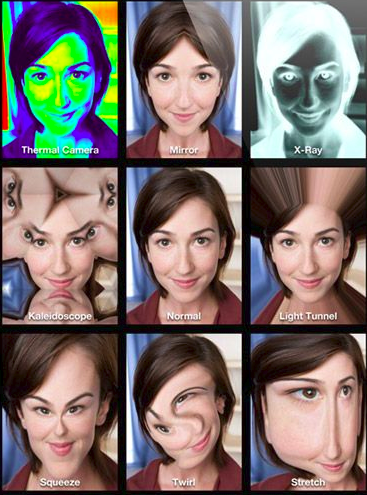
\includegraphics[width=0.3\textwidth]{images/photoBooth.png}
    \caption{Image editing using PhotoBooth application.}
    \label{fig:photoBooth}
\end{figure}

\subsection{Business Case and Financial Analysis }

Our product is new in the market, which makes our business case a great one. We can provide our services in two forms as following:
\begin{itemize}
    \item The first is being a software service that is used in police stations, so that any missing people or theft happens, they enters the description of potential suspects, so they can have an image of him/her to be able to find him faster. Also, it can be used in historical institutions that is responsible for finding information about historical characters and events from ancient descriptions.
    \item The second one is a website for general users to be able to use it for entertainment purposes or, for example, to generate images of their ancestors from description, so they get the chance to see them.
\end{itemize}

This means that we have three ways to earn money from our application :
\begin{itemize}
    \item The first way is the money paid by the institutions that uses the application for specific purposes (e.g. police stations or historical researches).
    \item The second way is the money paid by the users, who will be willing to be premium subscribers in the application. Premium subscription can give the user more server resources for faster generation and manipulation, as well as more number of generated faces per month.
    \item The third way is the companies that are interested to place their advertisements on our product.
\end{itemize}

So, we are going to address those three aspects in this section. In the business case, we will show the expected number of product sales over the next 5 years and how we will tune the price to counter the competition. Table \ref{tab:business} shows the business case study.

\begin{table}[H]
\centering
\caption{Business Case over 5 years.}
\begin{tabular}[t]{| l | l | l | l | l | l |}
\hline
Years & Year 1 & Year 2 & Year 3 & Year 4 & Year 5 \\
\hline
Avg Number of Customers & 30 & 50 & 100 & 120 & 200 \\
\hline
Product Purchase & \$1500 & \$1500 & \$2000 & \$2300 & \$2800 \\
\hline
Avg Number of Premium Subscribers & 200 & 500 & 800 & 1100 & 1500 \\
\hline
Premium Subscription Cost & \$5 & \$7 & \$12 & \$15 & \$20 \\
\hline
Average Ads earnings (per day) & \$1 & \$1 & \$3 & \$5 & \$8 \\
\hline
Average usage dayes per year & 100 & 170 & 200 & 180 & 210 \\
\hline
Average Profits from Ads & \$100 & \$170 & \$600 & \$900 & \$1680 \\
\hline
Average Profits from Subscription & \$1000 & \$3500 & \$9600 & \$16500 & \$30000 \\
\hline
Profits from Purchasing & \$45000 & \$75000 & \$200000 & \$276000 & \$560000 \\
\hline
Total Profits & \$46100 & \$78670 & \$210200 & \$293400 & \$591680 \\
\hline
\end{tabular}
\label{tab:business}
\end{table}

\newpage

Based on a business case study and the specifications needed, the cost estimation of our software as a service in a specific institution is the cost behind the hardware. Our application takes around 1 second on an \emph{Nvidia GTX 1080 ti} for generating the face from any description, but this can extend to be multiple seconds based on the connection. The whole system can be deployed on single PC with 11GB VRAM, around 700\$ for the GPU and 1500\$ to 2000\$ for the whole PC. For scalability, we can use 2 PCs one for generation and the other for Pose estimation to host the whole application. Also, we can scale out our system on more than 2 PCs for improved request parallelism. So, we can conclude the \emph{Capex} as shown in table \ref{tab:capex} and \emph{Opex} as shown in table \ref{tab:opex}. Given this information, we can construct the financial analysis as shown in table \ref{tab:cash_flow}.

\begin{table}[H]
\centering
\caption{Capex Table.}
\begin{tabular}[t]{| l | l |}
\hline
Items and Supplies & Cost \\
\hline
 Office Preparation ( offices, chairs , etc )&  \$5000  \\
\hline
 PCs and Laptops & \$10000 \\
\hline
Servers & \$3000 \\
\hline
Total Capex & \$18000 \\
\hline
\end{tabular}
\label{tab:capex}
\end{table}

\begin{table}[H]
\centering
\caption{Opex Table.}
\begin{tabular}[t]{| l | l |}
\hline
Items and Supplies & Cost per month \\
\hline
Salaries & \$4500 \\
\hline
Rent & \$400 \\
\hline
Bills ( electricity , water, etc ) & \$450\\
\hline
Total Opex & \$5350 \\
\hline
\end{tabular}
\label{tab:opex}
\end{table}

\begin{table}[H]
\centering
\caption{Cash flow Table over a year (in dollars)}
\begin{adjustbox}{angle=90}
\begin{tabular}[t]{ | l | l | l | l | l | l | l | l | l | l | l | l | l |}
\hline
 & Jan & Feb & Mar & Apr & May & June & July & Aug & Sep & Oct & Nov & Dec \\
\hline
\multicolumn{13}{|c|}{Capex}  \\
\hline
Office Equipment & 416 & 416 & 416 & 416 & 416 & 416 & 416 & 416 & 416 & 416 & 416 & 416 \\
\hline
Laptops and PCs & 833 & 833 & 833 & 833 & 833 & 833 & 833 & 833 & 833 & 833 & 833 & 833 \\
\hline
Servers & 250 & 250 & 250 & 250 & 250 & 250 & 250 & 250 & 250 & 250 & 250 & 250 \\
\hline
\multicolumn{13}{|c|}{Opex}  \\
\hline
Salaries & 4500 & 4500 & 4500 & 4500 & 4500 & 4500 & 4500 & 4500 & 4500 & 4500 & 4500 & 4500 \\
\hline
Rent & 400 & 400 & 400 & 400 & 400 & 400 & 400 & 400 & 400 & 400 & 400 & 400 \\
\hline
Bills & 450 & 450 & 450 & 450 & 450 & 450 & 450 & 450 & 450 & 450 & 450 & 450 \\
\hline
Sub Total & 6849 & 6849 & 6849 & 6849 & 6849 & 6849 & 6849 & 6849 & 6849 & 6849 & 6849 & 6849 \\
\hline
Accumulative & 6849 & 13698 & 20547 & 27396 & 34245 & 41094 & 47943 & 54792 & 61641 & 68490 & 75339 & 82188 \\
\hline
\multicolumn{13}{|c|}{Revenue}  \\
\hline
Purchasing & 5800 & 6500 & 7500 & 8000 & 5600 & 7000 & 6000 & 6500 & 5800 & 6800 & 7200 & 6700 \\
\hline
Subscription & 100 & 150 & 180 & 200 & 220 & 180 & 230 & 180 & 200 & 150 & 180 & 190 \\
\hline
Ads & 50 & 75 & 80 & 80 & 90 & 88 & 74 & 100 & 110 & 80 & 98 & 88 \\
\hline
Sub Total  & 5950 & 6725 & 7760 & 8280 & 5910 & 7268 & 6304 & 6780 & 6110 & 7030 & 7478 & 6978 \\
\hline
Accumulative & 5950 & 12675 & 20435 & 28715 & 34625 & 41893 & 48197 & 54977 & 61087 & 68117 & 75595 & 82573 \\
\hline
Profits & -899 & -1023 & -112 & 1319 & 380 & 799 & 254 & 185 & -554 & -373 & 256 & 385 \\
\hline
Taxes & - & - & - & 329.75 & 95 & 199.75 & 63.5 & 46.25 & - & - & 64 & 96.25 \\
\hline
Net Profits & -899 & -1023 & -112 & 989.25 & 285 & 599.25 & 190.5 & 138.75 & -554 & -373 & 192 & 288.75 \\
\hline
\end{tabular}
\end{adjustbox}
\label{tab:cash_flow}
\end{table}
